\chapter{Model Architecture} 
\label{ModelArchitecture}

Arguably, the most important aspect of a system based on deep neural networks, is the network architecture.  Year over year improvement in performance of DNNs in field of computer vision in recent years, was possible by using deeper and more sophisticated models. Figure \ref{fig:deeper} illustrates the number of layers in DNNs that won the ImageNet Large Scale Visual Recognition Challenge (ILSVRC) in recent years. 

\begin{figure}[h]
    \centering
    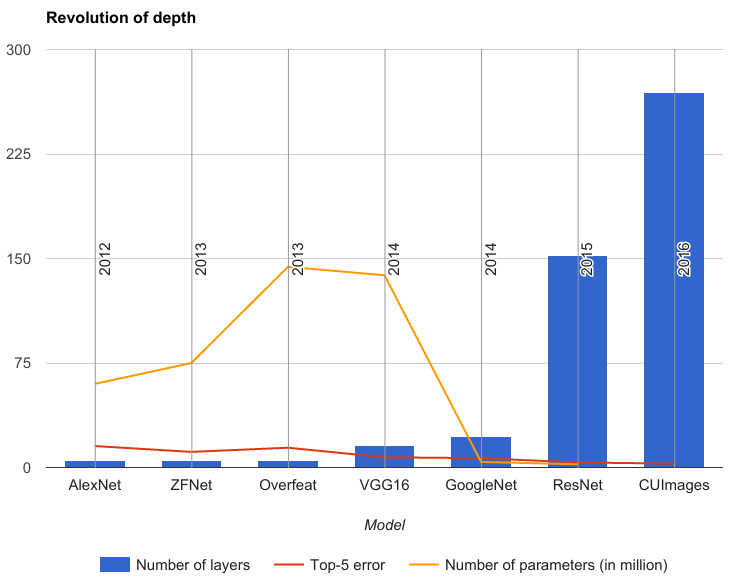
\includegraphics[scale=0.45]{Deeper}
    \caption{Evolution of depth, error-rate, and number of parameters in best-performing DNNs in ILSVRC Challenge over the years \caplicense{Diagram courtesy of https://medium.com/@pierre.ecarlat}}
    \label{fig:deeper}
\end{figure}

In this project three main types of network architectures were implemented: Baseline, VGG16, and ResNet50. Afterwards, various modifications to the architecture of these networks were investigated. The outcome of each experiment was used to guide the process of designing new modified versions of the network.  The architecture of these networks are discussed in next sections. 

\section{Baseline}

Based on the top-down sub-network of \citeauthor*{wang} \cite{wang}, a seven layer convolutional neural network was designed as the baseline model. Table \ref{tab:baseline} illustrates the architecture of this network. 

\pagebreak

\begin{table}[h]
\centering
\begin{tabular}{ccccc}
Layer Type & Number of Filters/Units & Size & Stride & Output Shape \\
\hline
Input &  &  &  & 240x320x3 \\
Convolution & 64 & 5x5 & 1x1 & 240x320x64 \\
Max Pooling &  & 2x2 & 2x2 & 120x160x64 \\
Convolution & 192 & 3x3 & 1x1 & 120x160x192 \\
Max Pooling &  & 2x2 & 2x2 & 60x80x192 \\
Convolution & 384 & 3x3 & 1x1 & 60x80x384 \\
Convolution & 256 & 3x3 & 1x1 & 60x80x256 \\
Convolution & 3 & 3x3 & 1x1 & 60x80x3 \\
Flatten &  &  &  & 14400 \\
Fully-Connected & 4096 &  &  & 4096 \\
Fully-Connected & 14400 &  &  & 14400 \\
Reshape &  &  &  & 60x80x3 \\
Resize &  &  &  &  240x320x3 \\
Normalise &  &  &  &  240x320x3 \\
\end{tabular}
\caption{Baseline network architecture}
\label{tab:baseline}
\end{table}

The input image passes through five convolution and two pooling layers. The output is flattened to a vector with size of 14400. Then, two fully connected layers are applied. The output of fully connected layers is reshaped to a tensor with size of 60x80x3. A bi-linear resizing layer, upsamples the output of the network to size of 240x320x3. Finally, the estimated values for the normal map are normalised by last layer of the network. 

Based on this architecture, several modified versions of the network were designed and the effect of these modifications on the results was investigated. These modifications are discussed as follows:

\subsection{Number of Convolution Filters}

Number of filters in convolutional layers is a parameter that affects the number of features extracted from input data. One can hypothesise that by estimating the normal maps based on more features, the performance of the network might increases. 

To investigate the effect of this parameter on output, the number of filters in last convolutional layer was increased from three to the maximum possible value. The other parameters in the network was kept as before. This decision was made because not only increasing the number of filters in other convolutional layers was not possible due to memory constraints, but more importantly, the main bottleneck in number of extracted features accessible to fully connected layers for normal estimation was the last convolutional layer. 

Unfortunately, because of memory constraints (12GB GPU Memory), having more than twelve filters at last convolutional layer was not possible. As mentioned before, fully connected layers have weighted connections to all feature maps of the last convolutional layer. Therefore, increase in number of these filters largely affects the total number of weights in the network and consequently memory usage.

\subsection{Size of Convolution Filters}

Another parameter that affects the extracted feature maps of the network, is the size of the convolution kernels. Larger kernels compute the value of feature maps at each location, based on a larger spatial neighbourhood. Estimating the normals by considering a bigger spatial region might produce more consistent outputs in each local neighbourhood and less noise in result. Although, there is a higher chance that local out-liners (e.g. at edge of an object) affect the neighbouring regions. 

In this model, the kernel size of the last convolutional layer in baseline architecture, was increased from 3x3 to 15x15. All other parameters were kept same as baseline model except the size of the padding at last convolutional layer. By using a larger padding, the shape of the output was kept the same size as baseline model (i.e. 60x80x3).

\subsection{Average Pooling}

As mention in section \ref{sec:pooling}, one of the main reasons of using a pooling layer is to keep the memory usage in bound. The max pooling layers achieve this task by choosing the maximum values of the feature maps under their filter window and discarding the rest of data. Therefore, always the feature with strongest response dominates the result. 

Alternatively, using an average pooling layer and considering the weaker features, might result in including more details in representation of input data. Based on this speculation, all the max pooling layers in baseline architecture were replaced with average pooling layers in a new model. Because this change does not affect the output shape of the layer, all other parameters of model remained intact.   

\subsection{Structure of Fully Connected Layers}

Another component of the network is the fully connected layers. These layers play the important role of estimating surface normals based on the feature maps provided by convolutional layers. Therefore, to have better outputs, it is important to have fully connected layers with carefully designed structure. 

The baseline model has two fully connected layers and thus there are two ways to modify its structure. Two separate models were designed; each with the goal of maximising the number of neurons in one of the fully connected layers. The models were executed several times to find the maximum number of neurons that fit in the memory. 

In one model, the number of neurons in last fully connected layer was increased from 14,400 to 57,600 neurons. By having a bigger outer fully connected layer, the resolution of output normal maps increases. Higher resolution output might increase the accuracy of results in a very good performing model, but it was expected to result in worse performance in our baseline model; because the model needs to produce more estimated values based on limited input from previous layer. Also, the resize layer in the network was accordingly modified to keep the overall output shape of the network the same as baseline model. 

In the alternative model, the number of neurons in first fully connected layer was increased from 4,096 to 14,400. Hypothetically, a bigger inner fully connected layer can pass more information from convolutional layers to other fully connected layers. By doing so, it might be possible that this extra information improve the output of the network. Because of memory constraints, the last fully connected layer could not be bigger than 6,480 neurons. While this problem affects the comparison of this model to the baseline model, the results are still comparable to the other model.

\subsection{Up-Sampling}

The up-sampling layer in baseline model, increases the resolution of the output by applying the bi-linear up-sampling method. Bi-linear up-sampling is a simple method that produces acceptable results and is used in other related work discussed in section \ref{sec:relatedwork}. There are also other up-sampling methods such as nearest neighbour, and cubic spline interpolation available for use in this layer.  

To explore the effect of using a different up-sampling method on final results, a model with simpler up-sampling layer was implemented. In this layer up-sampling was performed by simply repeating the values. The motivation for using a simpler up-sampling method is that the other layers of the network do not need to learn how to deal with more complex transformations performed by bi-linear up-sampling layer.  

\subsection{Replacing a Fully Connected Layer with Convolutional Layer}

In some applications in the field of computer vision, the fully convolutional neural networks have achieved considerable results. These networks only rely on use of convolutional/pooling layers and do not have any fully connected layers. Based on this idea, a modified network architecture was implemented. 

In this model, the first fully connected layer was removed and the size of the filters in last convolutional layer was changed from 3x3 to 1x1. By doing so, the last convolutional layer acts on each individual value on the feature maps. 

\section{VGG16}

VGG16 \cite{vgg}, is a very popular network architecture in many computer vision tasks. Therefore, this network was used as a basis for another group of network architectures that were explored for the task of surface normal estimation. First, the original network architecture was adapted for use in this project. Table \ref{tab:vgg} illustrates this architecture. 

\begin{table}[h]
\centering
\begin{tabular}{cccccc}
Block No. & Layer Type & Filters/Units & Size & Stride & Output Shape \\
\hline
\hline
 & Input &  &  &  & 240x320x3 \\
 \hline
\multirow{3}{3em}{Block 1} & Convolution & 64 & 3x3 & 1x1 & 240x320x64 \\
 & Convolution & 64 & 3x3 & 1x1 & 240x320x64 \\
 & Max Pooling &  & 2x2 & 2x2 & 120x160x64 \\
 \hline
\multirow{3}{3em}{Block 2} & Convolution & 128 & 3x3 & 1x1 & 120x160x128 \\
 & Convolution & 128 & 3x3 & 1x1 & 120x160x128 \\
 & Max Pooling &  & 2x2 & 2x2 & 60x80x128 \\
 \hline
\multirow{4}{3em}{Block 3} & Convolution & 256 & 3x3 & 1x1 & 60x80x256 \\
 & Convolution & 256 & 3x3 & 1x1 & 60x80x256 \\
 & Convolution & 256 & 3x3 & 1x1 & 60x80x256 \\
 & Max Pooling &  & 2x2 & 2x2 & 30x40x256 \\
 \hline
\multirow{4}{3em}{Block 4} & Convolution & 512 & 3x3 & 1x1 & 30x40x512 \\
 & Convolution & 512 & 3x3 & 1x1 & 30x40x512 \\
 & Convolution & 512 & 3x3 & 1x1 & 30x40x512 \\
 & Max Pooling &  & 2x2 & 2x2 & 15x20x512 \\
 \hline
\multirow{4}{3em}{Block 5} & Convolution & 512 & 3x3 & 1x1 & 15x20x512 \\
 & Convolution & 512 & 3x3 & 1x1 & 15x20x512 \\
 & Convolution & 512 & 3x3 & 1x1 & 15x20x512 \\
 & Max Pooling &  & 2x2 & 2x2 & 7x10x512 \\
 \hline
 & Flatten &  &  &  & 35840 \\
 & Fully-Connected & 4096 &  &  & 4096 \\
 & Fully-Connected & 14400 &  &  & 14400 \\
 & Reshape &  &  &  & 60x80x3 \\
 & Resize &  &  &  &  240x320x3 \\
 & Normalise &  &  &  &  240x320x3 \\
\end{tabular}
\caption{Adapted VGG16 network architecture}
\label{tab:vgg}
\end{table}

The parameters of the network were initialised based on a VGG16 model trained on ImageNet data set. Each block of this network extracts features with a different level of abstraction. To investigate the effect of using different levels of data representation abstraction in output of the network, three different models were implemented. In addition to these models, a network architecture that concatenates the different levels of abstraction was also designed. These models are discussed as follows.

\subsection{Models Based on the Low, Mid, and High Parts of the VGG16}

The first model was designed based on the output from the lower blocks of the VGG16 architecture. In this model only the block 1 and block 2 of the original VGG16 network was implemented. After the last layer of the block 2, a convolutional layer with 12 filters (size of 3x3) was applied and the output was flattened and passed to the fully connected layers. Considering the relatively large size of the feature maps in block 2, it was not feasible to include more than 12 filters in the last convolutional layer due to memory constraints. 

The next model also included the block 3 layers. Likewise, a convolutional layer connected the output of the last pooling layer to the flattening layer. This time, 48 filters in the last concolutional layer was the maximum number of filters that fit in memory. 

Finally, the last model implemented the blocks 1 to 4 of the VGG16 architecture. The additional convolutional layer had 192 filters with size of 3x3. The outputs of these models were compared to the results of the adapted VGG16 model.  

\subsection{Concatenating the Low, Mid, and High Parts of the VGG16}

Inspired by the work of \citeauthor*{bansal} \cite{bansal}, a new network architecture based on VGG16 was designed. This model included all the convolutional/pooling layers of the original VGG16 network; but, instead of connecting the last pooling layer of the network to the flattening layer, the feature maps from the last convolutional layers of all blocks were concatenated and passed to an additional convolutional layer with 12 filters. Figure \ref{fig:vggconcat} illustrates the architecture of this network.

Hypothetically, by using feature maps with different levels of abstraction, the fully connected layers have access to a much richer data representation. Therefore, a better performance might be achievable. A problem with using the output of different layers is the difference between the size of feature maps. To solve this problem, additional pooling layers were applied on the outputs of block 1 and 2, and the outputs of block 4 and 5 were up-sampled to size of 60x80x3. 

\begin{figure}
    \centering
    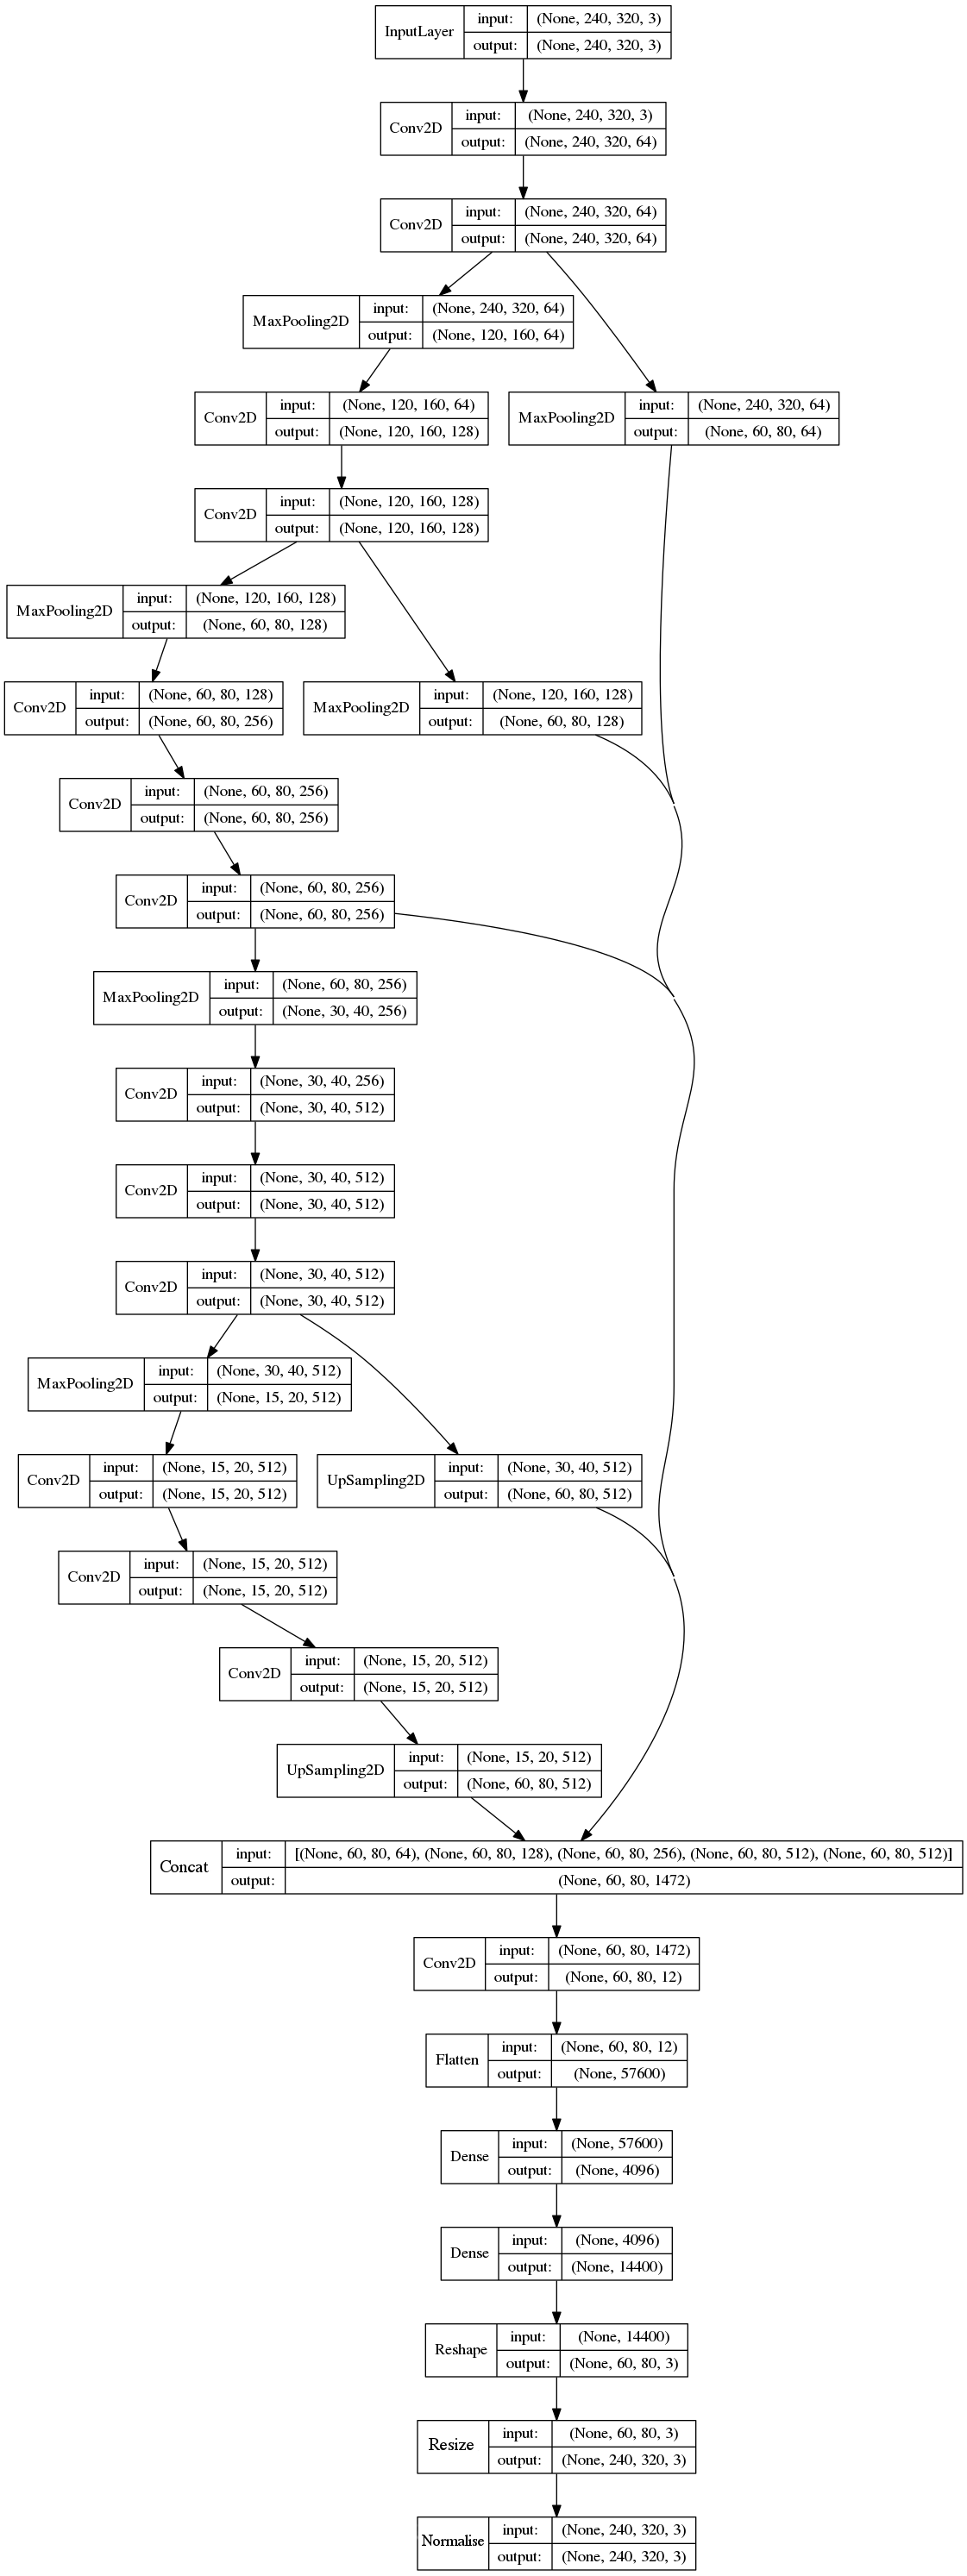
\includegraphics[height=\dimexpr \textheight-25pt]{VGGConcat}
    \caption{Network architecture based on the concatenation of feature maps from different layers}
    \label{fig:vggconcat}
\end{figure}

\section{ResNet50}

ResNet \cite{resnet} is another popular deep neural network in computer vision tasks over the last few years. This network is based on the concept of Residual blocks. The general structure of a residual block is illustrated in figure \ref{fig:resblock}. The right path in the block is referred to as shortcut. By using this structure, training very deep neural networks is possible. Using several variations of residual blocks in a network is a common practice. 

\begin{figure}[h]
    \centering
    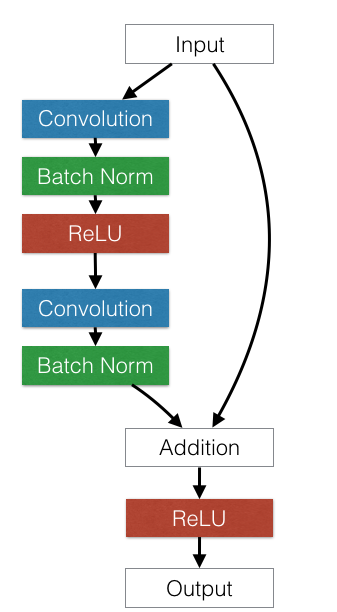
\includegraphics[scale=0.45]{ResBlock}
    \caption{A residual block in ResNet network architecture \\caplicense{Diagram courtesy of \url{https://leonardoaraujosantos.gitbooks.io/artificial-inteligence/}}}
    \label{fig:resblock}
\end{figure}

In this project a ResNet-based network architecture with 50 layers was adapted to the task of surface normal estimation. Two variations of residual blocks were used: 

\begin{itemize}
    \item \emph{Identity Residual Block}: three convolutional layers and a shortcut path
    \item \emph{Convolutional Residual Block}: three convolutional layers and a convolutional layer on the shortcut path
\end{itemize}

As illustrated in table \ref{tab:resnet}, four convolutional and twelve identity residual blocks were used in the architecture of this network. For the last pooling layer, an average pooling was chosen. Finally, the same structure as the baseline model was used for the upper layers of the network.

Given enough training samples, a complex network such as ResNet50, could potentially achieve good results. The performance of this network was explored in this project.

\begin{table}[h]
\centering
\begin{tabular}{c}
Type of Component \\
\hline
Input Layer \\
Convolutional Layer \\
Max Pooling Layer \\
Convolutional Residual Block \\
Identity Residual Block \\
Identity Residual Block \\
Convolutional Residual Block \\
Identity Residual Block \\
Identity Residual Block \\
Identity Residual Block \\
Convolutional Residual Block \\
Identity Residual Block \\
Identity Residual Block \\
Identity Residual Block \\
Identity Residual Block \\
Identity Residual Block \\
Convolutional Residual Block \\
Identity Residual Block \\
Identity Residual Block \\
Average Pooling Layer \\
Flattening Layer \\
Fully-Connected Layer \\
Fully-Connected Layer \\
Reshaping Layer \\
Resizing Layer \\
Normalisation Layer\\
\end{tabular}
\caption{Adapted ResNet50 network architecture}
\label{tab:resnet}
\end{table} 